\documentclass[../dissertation.tex]{subfiles}
 
\begin{document}

\section{Experiment 1}

The goals for this experiment were twofold. First, I hoped to test order effects in a paradigm originally designed to test a dual-systems model of categorization. Despite the fact that many approaches posit such a model, only one approach (COVIS) has explicitly tested how a given individual switches between systems for categorization (e.g., \citealp{Ashby2010, Erickson2008}, described above). Most other studies that compare different types of categorization do so in a between-subjects manner (e.g., \citealp{Kloos2008}). Thus, this study is one of the first to look at the relationship between two categorization systems using a non-COVIS within-subjects design. This task is also the first to test how individual differences in language ability modulate this relationship. \par
	This experiment also has a more practical purpose. One of the overarching goals of this dissertation is to compare different paradigms of category learning. However, all studies using a statistical density approach have been done between subjects, so we do not yet know if there are any transfer effects for this type of task. In addition, no studies to date have tested for transfer effects along the spectrum of language ability. This experiment carefully conducts three order analyses to fully understand the statistical density category learning task. This will benefit both  practical understanding of this task as well as its underlying theoretical framework. \par
	An interesting feature of the statistical density task is its two manipulations, each of which engages or requires one of the two category learning systems. First, the instruction type engages either the associative or the hypothesis-testing system by placing different task demands. Second, the stimulus requires a certain category learning system. Recall that dense and sparse stimuli are best learned by different systems. Thus, each block can either be a match (where the instruction type engages the ideal system for the stimulus type) or a mismatch (where the instruction type engages the wrong system for the stimulus type). \par 
	To fully understand this task, I tested for order effects in both matching and mismatching conditions. First, I tested order for the matching conditions. This analysis is the most simple and straightforward test of order; can participants switch between systems when both the stimulus type and the learning type cue a certain system? The second order analysis tested dense stimuli to see whether participants were able to engage the associative system even when the learning instructions sometimes cued the hypothesis-testing system. Further, if participants were unable to overcome the learning instructions and ended up using the hypothesis-testing system in their first block, this analysis investigated whether they could switch to the associative system in subsequent blocks following task demands. Finally, the third order analysis tested sparse stimuli. Similarly, I tested whether participants could engage the hypothesis-testing system to learn sparse stimuli even when task demands cued the associative system. This order analysis also tested the participants' ability to subsequently switch away from the associative system. \par
	
\subsection{Method}
\subsubsection{Participants}
\begin{wraptable}[7]{R}{0.35\linewidth}
\vspace{-10pt}
\caption{Group sizes for each order.}
\vspace{-10pt}
\begin{center}
\begin{tabularx}{0.35\textwidth}{ YYY } 
 \toprule
 Analysis & Group & \textit{N} \\ 
 \midrule
 \multirow{2}{*}{1} & 1 & 40 \\ 
 & 2 & 38 \\ 
  \midrule
  \multirow{2}{*}{2} & 3 & 39 \\ 
 & 4 & 39 \\
  \midrule
  \multirow{2}{*}{3} & 5 & 36\\ 
 & 6 & 37 \\ 
 \bottomrule
\end{tabularx}
\end{center}
\label{exp1Ns}
\end{wraptable} Data was collected from 236 undergraduate psychology students at the University of Connecticut (161 Female, 67 Male, mean age = 18.94). Data for the category learning task was lost for 7 subjects due to technical errors, which led to slightly unequal group sizes. The final sample size was 229. Each subject was placed into one of six groups. Each group completed two blocks of the category learning task in a specific order (described below in detail).

\subsubsection{Category learning task}
	This task measures learning of dense and sparse categories. It is based off of a paradigm from previous research \citep{Kloos2008}. Participants learn novel categories of items in four conditions stemming from a 2 (learning type) x 2 (stimulus type) design. Table \ref{stimsystems} summarizes how each experimental manipulation corresponds to the theorized category learning systems. Learning type can be either supervised or unsupervised. In \textit{supervised} learning, participants learn the categories by being instructed on the relevant features (e.g., “All friendly aliens have big noses.”). Images of the relevant features are provided along with the descriptions. In \textit{unsupervised} learning, participants learn the categories by viewing sixteen instances of the category.  \par
	
\begin{wraptable}[6]{L}{0.7\linewidth}
\vspace{-10pt}
\caption{Relationship between learning systems and experimental manipulations.}
\vspace{-10pt}
\begin{center}
\begin{tabularx}{0.7\textwidth}{ YYY } 
 \toprule
Experimental feature & Hypothesis-testing & Associative  \\
 \midrule
Learning type        & Supervised         & Unsupervised \\
Stimulus type        & Sparse             & Dense  \\ 
 \bottomrule       
\end{tabularx}
\label{stimsystems}
\end{center}
\end{wraptable}

	Categories in this experiment can either be sparse or dense. Category density ranges from zero (where all features vary freely) to one (where all features co-occur perfectly), based on a comparison between within- and between-category entropy \citep{Sloutsky2010}. All categories in this experiment have seven dimensions. The \textit{sparse} categories cohere on a single dimension, while the other dimensions vary freely (density = .25). In contrast, the \textit{dense} categories cohere on six of the seven dimensions (density = .75). The seventh dimension is allowed to vary freely. For more details on how density was calculated, see Appendix A. Stimuli for each of the four blocks are different. For example stimuli, see Appendix B.  \par
	
\begin{wraptable}[8]{R}{0.65\linewidth}
\vspace{-10pt}
\caption{Block orders for statistical density task.}
\vspace{-10pt}
\begin{center}
\begin{tabular}{cccc}
 \toprule
 Analysis & Group & First Block & Second Block \\ 
 \midrule
 \multirow{2}{*}{1} & 1 & Unsupervised-dense & Supervised-sparse \\ 
 & 2 & Supervised-sparse & Unsupervised-dense \\ 
 \midrule
  \multirow{2}{*}{2} & 3 & Unsupervised-dense & Supervised-dense \\ 
 & 4 & Supervised-dense & Unsupervised-dense \\
 \midrule
  \multirow{2}{*}{3} & 5 & Unsupervised-sparse & Supervised-sparse \\ 
 & 6 & Supervised-sparse & Unsupervised-sparse \\ 
 \bottomrule 
\end{tabular}
\end{center}
\vspace{-20pt}
\label{exp1order}
\end{wraptable} \par

	This task is within-subjects. Based on the group they were placed into, participants completed two of the four possible learning-category type combinations. In this experiment, I conducted three different order analyses. This design led to six possible order groups that each participant could be placed into (see Table \ref{exp1order}). \par
 In each block, participants were introduced to the task through a short cover story. They were told to learn which items go with a certain property (e.g., which aliens are friendly). Crucially, no labels were attached to the categories (e.g., some aliens are Ziblets). Then, participants completed a training block (supervised or unsupervised; see Fig. \ref{sloutskytraining}). 

\begin{figure}[h]
\begin{center}
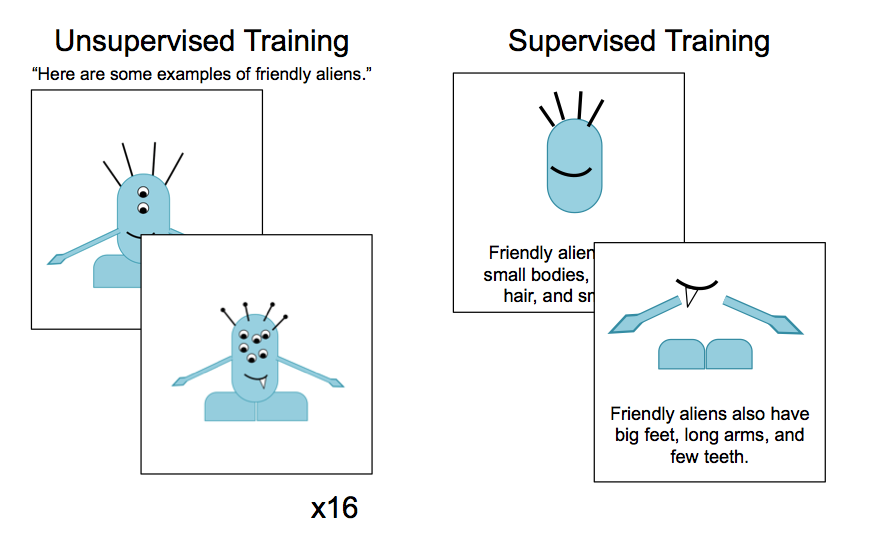
\includegraphics[scale=0.5]{sloutsky_training}
\caption[Training conditions in category learning task]{Examples of the learning type manipulation for the category learning task.}
\vspace{-10pt}
\label{sloutskytraining}
\end{center}
\end{figure}
 
 
 During training, only members of the target category or its features were shown. After training, participants completed 40 test trials (16 target, 16 distractor, 8 catch). In each test trial, participants saw a single item and used the keyboard to indicate whether the item matched the category they had just learned (e.g., if the alien is friendly). Catch items looked significantly different than both the target and competing categories, so participants should have always rejected them as members of the learned category. This experiment was presented using PsychoPy v.1.84.2 \citep{Peirce2007}. \par
 
\subsubsection{Behavioral measures}
	I used multiple assessments to test participants' language ability.  The choice of assessments was based on the epiSLI criteria for language impairment \citep{Tomblin1996}, which includes comprehension, expression, vocabulary, grammar, and narrative. I adapted these requirements from a kindergarten population to a college-aged population. The epiSLI criteria have been shown to be robust for diagnosis of specific language impairment (SLI). In addition, other studies of language impairment more broadly have adapted a similar multidimensional approach to measuring language ability, sometimes including measures of phonological skills \citep{Catts2006}. Thus, using assessments that cover the many domains of language outlined in epiSLI criteria allowed me to get a fuller picture of individual differences in language ability. See Table \ref{slitable} for a summary of the assessments and which domains of the epiSLI criteria they cover. The specific tests used in this experiment are detailed below. \par
	\textbf{Test of word reading efficiency (TOWRE) phonemic decoding subtest.} TOWRE is a test of nonword fluency \citep{Torgesen1992}. This test is a part of the comprehension aspect of epiSLI, since the comprehension measure is reading-based \citep{Gough1986a}. In this subtest of the TOWRE, individuals have 45 seconds to read as many nonwords as possible. The nonwords become longer and more difficult as the list goes on. The raw score from the TOWRE was calculated by counting the number of words correctly pronounced before the time limit. These raw scores were then converted to standard scores using age-based norms. The standard scores for this task are based on a distribution with a mean of 100 and a standard deviation of 15. In the current age range, a perfect raw score (63) on the TOWRE returns a standard score of "\textgreater 120." For the purposes of this study, scores of "\textgreater 120" were trimmed to 120. \par
	\textbf{Woodcock Johnson-III word attack (WA) subtest.} This task measures nonword decoding accuracy \citep{Woodcock2001}. Like the TOWRE, it is helpful for measuring the comprehension aspect of epiSLI. Participants read a list of nonwords out loud at their own pace. Raw scores were calculated by counting the number of words the participant said correctly. Raw scores were converted to standard scores using age-based norms. The standard score distribution has a mean of 100 and a standard deviation of 15. \par
	\textbf{Computerized reading comprehension.} This test covers the comprehension and narrative aspects of epiSLI. This computerized reading comprehension (CRC) test is based on the Kaufman Test of Educational Achievement (KTEA) reading comprehension subtest \citep{Kaufman2004}. To create this test, I copied the passages and questions contained in the KTEA reading comprehension subtest into E-Prime \citep{schneider2002prime} for presentation on a computer. Then, I created multiple choice answers for the KTEA questions that did not already have them. In this task, participants read short expository and narrative texts and answered multiple-choice comprehension questions about them. Some questions were literal, while others required participants to make an inference. Participants completed as many questions as they could in 10 minutes. Once 10 minutes had elapsed, the participant was allowed to answer the question currently on the screen and then the assessment closed. Because this task is a modified version of the KTEA, I used raw scores in analysis rather than standardized scores based on the KTEA norms. Raw scores were calculated by counting the number of correctly answered questions for each participant.  \par
	
\begin{wraptable}[8]{R}{0.5\linewidth}
\caption{Assessments of language and their corresponding epiSLI domains.}
\vspace{-10pt}
\begin{center}
\begin{tabular}{ cc } 
 \toprule
 Test & epiSLI Criteria \\ 
 \midrule
 TOWRE & \multirow{2}{*}{Comprehension (decoding aspect)}\\ 
 WA & \\ 
 CRC & Comprehension, narrative \\
 ND Vocab & Vocabulary \\ 
 CELF RS & Grammar, expression \\ 
 \bottomrule 
\end{tabular}
\end{center}
\label{slitable}
\end{wraptable}

	\textbf{Nelson-Denny vocabulary subtest.} The Nelson-Denny vocabulary subtest is a written assessment of vocabulary \citep{Brown1981}. This test covers the vocabulary aspect of epiSLI. It has been used in multiple studies of college-aged adults and provides sufficient variability for individual difference investigations in this population \citetext{e.g., \citealt{Boudewyn2015}; \citealt{Stafura2014}}. Participants were asked to choose the word closest to a target vocabulary word for 80 total items. Participants were allowed unlimited time to complete all items. Raw scores were generated by counting the total number of correctly answered items. The raw scores were then converted to standard scores based upon a norming sample including students in 10th, 11th, and 12th grade as well as two- and four-year college students. The standard scores for this assessment have a mean of 200 and a standard deviation of 25. \par
	\textbf{Clinical Evaluation of Language Fundamentals recalling sentences subtest.} I used the Recalling Sentences subtest from the Clinical Evaluation of Language Fundamentals - Fourth Edition \citetext{CELF; \citealt{Semel2006}} to cover the grammar and expression aspects of epiSLI. Participants heard sentences and were asked to repeat them. Scoring was based on how many errors the participant made in their repetition. Raw scores were calculated by adding up the number of points achieved for each item. These were then converted to standard scores using age-based norms. The standard scores are based on a distribution with a mean of 10 and a standard deviation of 3. \par
	\textbf{Raven's Advanced Matrices.} Finally, I used Set II of Raven's Advanced Matrices (RAM) to measure nonverbal IQ \citep{Raven1998}. In this task, participants saw a grid containing eight images and an empty space. The images were arranged in the grid according to some rule or rules. Participants chose one of eight additional images to fit in the empty space. Due to time constraints, I restricted participants to 10 minutes in this task. Since this administration is different than the standard administration, I did not use standard scores. Raw scores were calculated by counting the number of correct answers given within 10 minutes.

\subsubsection{Procedure}
	Each participant completed the category learning task as well as all of the behavioral measures. TOWRE, WA, and CELF were audio recorded to allow for offline scoring. To allow multiple subjects to be run in a single timeslot, some participants received tasks they could complete on their own (category learning, ND, computerized reading comprehension, Raven's) first while others completed tasks with the experimenter first (WA, CELF, TOWRE). Together, the seven tasks took approximately one hour.
	
\subsection{Results}

\subsubsection{Category learning task data processing}
	For basic descriptive statistics on the category learning task, see Table \ref{exp1expdesc}. To process the category learning task data, first all blocks where 5 or fewer catch items were correctly rejected were dropped from analysis. This resulted in 22 total missing blocks (out of 458 total), including both blocks from a single subject in group 5. For all analyses shown below, accuracy was converted to \textit{d'} values \citep{macmillan2004} using the R package \textbf{neuropsychology} \citep{neuropsych}. Correction for extreme values was done following \citet{Hautus1995}. For reaction time, all incorrect trials were discarded. Then, outliers were removed on a by-trial basis by calculating the mean and standard deviation of RTs within a given subject and block. Any trial with an RT more than 2 SDs away from the mean was discarded.   \par

\begin{table}[H]
\caption{Descriptive statistics for the category learning task.}
\vspace{-10pt}
\begin{center}
\begin{tabularx}{\textwidth}{>{\centering\arraybackslash}p{1.5cm}>{\centering\arraybackslash}p{1.5cm}YYY}
\toprule
Analysis       & Group              & Block               & Mean (SD) Accuracy & Mean (SD) RT (ms) \\ \midrule
\multirow{4}{*}{1} & \multirow{2}{*}{1} & Unsupervised-dense  & 0.91 (0.19)        & 958 (291)        \\  
                   &                    & Supervised-sparse   & 0.93 (0.14)        & 705 (291)         \\ \cline{2-5} 
                   & \multirow{2}{*}{2} & Supervised-sparse   & 0.72 (0.34)        & 759 (385)         \\  
                   &                    & Unsupervised-dense  & 0.90 (0.18)        & 742 (370)         \\ \midrule
\multirow{4}{*}{2} & \multirow{2}{*}{3} & Unsupervised-dense  & 0.91 (0.18)        & 963 (499)        \\  
                   &                    & Supervised-dense    & 0.91 (0.23)        & 834 (429)         \\ \cline{2-5} 
                   & \multirow{2}{*}{4} & Supervised-dense    & 0.90 (0.21)        & 854 (482)         \\  
                   &                    & Unsupervised-dense  & 0.92 (0.18)        & 777 (394)         \\ \midrule
\multirow{4}{*}{3} & \multirow{2}{*}{5} & Unsupervised-sparse & 0.57 (0.35)        & 1166 (600)        \\ 
                   &                    & Supervised-sparse   & 0.93 (0.14)        & 715 (311)         \\ \cline{2-5} 
                   & \multirow{2}{*}{6} & Supervised-sparse   & 0.93 (0.12)        & 752 (353)         \\ 
                   &                    & Unsupervised-sparse & 0.53 (0.38)        & 917 (470)        \\
 \bottomrule                    
\end{tabularx}
\label{exp1expdesc}
\end{center}
\end{table}

\subsubsection{Behavioral measures}
\begin{wraptable}[8]{r}{0.6\linewidth}
\begin{center}
\vspace{-20pt}
\caption{Descriptive statistics for behavioral measures}
\vspace{-10pt}
\begin{tabular}{Lccc}
 \toprule
Assessment                         & Mean & SD   & Range   \\
\midrule 
CELF Recalling Sentences SS        & 10.7 & 1.86 & 3-14    \\
Computerized Reading Comprehension & 21.7 & 5.12 & 7-48    \\
Nelson-Denny Vocabulary SS         & 229  & 14.0 & 175-255 \\
TOWRE SS                           & 96.2 & 9.86 & 59-120  \\
Word Attack SS                     & 99.7 & 9.04 & 75-120  \\
Raven's Advanced Matrices          & 15.1 & 4.58 & 0-26    \\
 \bottomrule 
\end{tabular}
\label{exp1behdesc}
\end{center}
\end{wraptable}
\par
	For basic descriptive statistics on the behavioral measures, see Table \ref{exp1behdesc}. Before performing any statistical analyses using these measures, I checked their normality using the D'Agostino normality test from the R package \textbf{fBasics} \citep{fBasics}. Four measures (CRC, ND Vocab, CELF RS, RAM) were significantly skewed. These measures were centered, scaled, and transformed using Yeo-Johnson transformations from R package \textbf{caret} \citep{caret}. The remaining measures (TOWRE, WA) were not skewed and thus were simply scaled and centered. \par
	Since my goal was to create a composite measure of language ability, I investigated the relationship between the behavioral measures. First, I constructed a correlation matrix between all of the behavioral measures (see Table \ref{exp1behcorr}). All pairs of measures had a significant positve correlation, with the exception of CELF RS and RAM. To further test whether the behavioral measures could be combined into a single composite, I ran a principal components analysis (PCA) on the 5 assessments related to epiSLI (i.e., all assessments except RAM). The Kaiser-Meyer-Olkin overall measure of sampling adequacy was 0.69, above the commonly accepted threshold of 0.6. Bartlett's test of sphericity was also significant $\chi^{2}(10)$  = 236.16, \textit{p} \textless 0.001. Both suggest that the 5 behavioral assessments were suitable for a PCA. \par
	The first component in the PCA accounted for 47.74\% of the variance and had an eigenvalue of 2.38. All of the factor loadings for this component were quite similar, ranging from -0.41 to -0.51. The second factor accounted for an additional 20.5\% of the variance and had an eigenvalue of 1.02. This factor separated the two measures involved in decoding (TOWRE and WA) from the other measures (CRC, ND Vocab, and CELF RS). The remaining components had eigenvalues below 1. Thus, of the two significant components, the first component explained almost half of the variance and had an eigenvalue more than double the second component, which largely represented decoding ability. Since the first component indicated that most of the measures loaded similarly, I decided to take a simple means approach to creating a language composite measure. \par
	The language composite measure was created by averaging the 5 scaled, centered, and/or transformed measures. For participants with missing behavioral measures, the composite was created by averaging the remaining available measures. No subject was missing more than 1 measure. This composite measure was then scaled but not centered. This language composite measure and the centered, scaled, and transformed RAM measure are used in the analyses investigating order effects reported below.


\begin{table}[H]
\caption{Correlations between behavioral measures.}
\vspace{-10pt}
\begin{center}
\begin{tabularx}{\textwidth}{p{7cm}YYYYYY}
\toprule
                                      & 1       & 2       & 3       & 4      & 5       & 6 \\
\midrule
1. Computerized Reading Comprehension & -       &         &         &        &         &   \\
2. Nelson-Denny Vocabulary            & 0.57*** & -       &         &        &         &   \\
3. CELF Recalling Sentences           & 0.31*** & 0.40*** & -       &        &         &   \\
4. Raven's Advanced Matrices          & 0.31*** & 0.34*** & 0.09    & -      &         &   \\
5. TOWRE                              & 0.22**  & 0.28*** & 0.26*** & 0.16*** & -       &   \\
6. Word Attack                        & 0.22**  & 0.38*** & 0.29*** & 0.22*** & 0.53*** & - \\
\bottomrule
\end{tabularx}
\label{exp1behcorr}
\end{center}
\small\textit{Note}. *\textit{p} \textless 0.05, **\textit{p} \textless 0.001, ***\textit{p} \textless 0.0001
\end{table}

		
\subsubsection{Order analysis 1: matching conditions}
	The first analysis investigated order effects for blocks in which the learning type (supervised vs. unsupervised) and category type (sparse vs. dense) both engaged the same category learning system (hypothesis testing vs. associative). Participants completed supervised-sparse (hypothesis-testing) and unsupervised-dense (associative) blocks.  \par

\begin{wrapfigure}{R}{0.55\textwidth}
\vspace{-10pt}
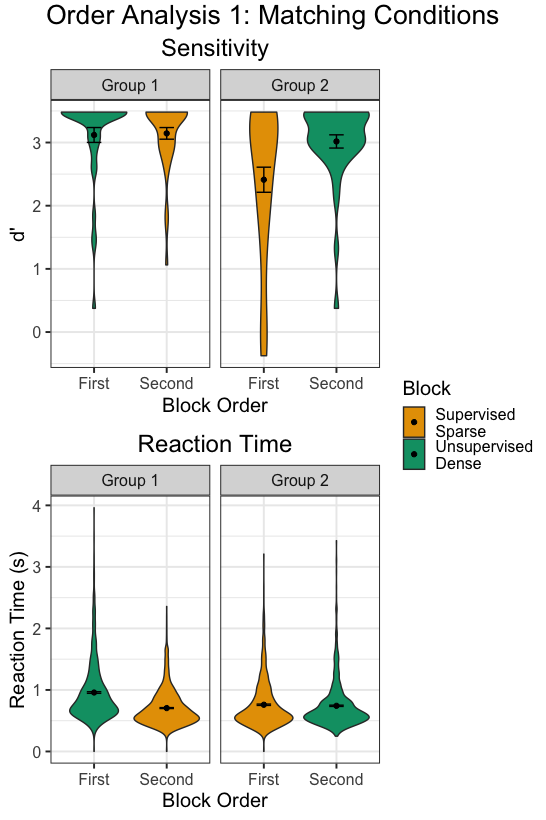
\includegraphics[scale=0.5]{oe1.png}
\caption[Sensitivity and reaction time for order analysis 1]{Sensitivity (d')  and reaction time for each block completed by each group for order analysis 1. Points indicate means with error bars reflecting standard error. Shaded portions represent the distribution of sensitivity or reaction time values.}
\label{oe1}
\vspace{-20pt}
\end{wrapfigure}		
	
	\textbf{Sensitivity.} I used linear mixed-effects models to examine the effects of block and order on sensitivity at test. Sensitivity in these models was measured by \textit{d'} values for each subject by block. The base model included random intercepts for subject. Adding block and order as fixed effects significantly increased model fit, $\chi^{2}(2)$ = 13.21,  \textit{p} = 0.001. Adding the interaction between block and order further improved model fit, $\chi^{2}(1)$ = 6.03,  \textit{p} = 0.014. Thus, the final model including only experimental conditions had fixed effects of block, order, and the interaction between block and order as well as random intercepts for subject. \par
	This model revealed two significant effects. First, there was a significant main effect of order, \textit{F}(1,75) = 8.60, \textit{p} = 0.004. There was also a significant interaction between block and order, \textit{F}(1,74) = 6.10, \textit{p} = 0.02. There was not a significant main effect of block, \textit{F}(1,76) = 2.61, \textit{p} = 0.11. The interaction was broken down by conducting two separate models for each of the orders (unsupervised-dense first and supervised-sparse first). These analyses showed that when the associative system was engaged first (unsupervised-dense first), there was no significant main effect of block, \textit{F}(1,36) = 0.014, \textit{p} = 0.91. When the hypothesis testing system was used first (supervised-sparse first), there was a significant effect of block, \textit{F}(1,37) = 7.52, \textit{p} = 0.009. This shows that when participants complete engage the hypothesis-testing system first, performance on the supervised-sparse (hypothesis-testing) block is lower than in the unsupervised-dense (associative) block. \par
	To investigate the effect of individual differences in language ability on the order effect, I used the final model above which included main effects for block and order as well as their interaction. I then added  the language composite measure as a fixed effect. I also added RAM to control for nonverbal IQ. This model revealed no significant effects for RAM or the language composite; there remained a significant interaction between block and order. \par
	\textbf{Reaction time}. Again, I used linear-mixed effects models to look at the effects of block and order on reaction time at test. While the sensitivity measure was at the block level, reaction time here is modeled at the item level. The base model included random intercepts for subject and for block nested within subject. Adding the fixed effects of block and order increased the model fit, $\chi^{2}(2)$ = 25.02,  \textit{p} \textless 0.001. Further, adding the interaction between block and order improved model fit, $\chi^{2}(1)$ = 33.11,  \textit{p} \textless 0.001. \par
	This model showed three significant effects. There was a significant main effect of block, \textit{F}(1,72) = 62.50, \textit{p} \textless 0.001. There was also a significant main effect of order, \textit{F}(1,77) = 4.17, \textit{p} = 0.04. Finally, there was a significant interaction between block and order, \textit{F}(1,72) = 40.49, \textit{p} \textless 0.001. To break down this interaction, I ran follow-up models for each of the two orders. This showed that when the associative system was engaged first (unsupervised-dense first), there was a significant main effect of block, \textit{F}(1,36) = 69.46, \textit{p} \textless 0.001. When the hypothesis testing system was used first (supervised-sparse first), there was no significant effect of block, \textit{F}(1,36) = 0.02, \textit{p} = 0.88. This result is the opposite of what was found in sensitivity. When the associative system is engaged first, there is a difference in reaction time between blocks, but when the hypothesis-testing system in engaged first, there is no difference in reaction time. \par
	Similar to the sensitivity analysis, I added RAM and language ability as fixed effects to the final reaction time model from above. Neither had any effect on reaction time. The main effects and interactions from above stayed significant. \par 
	\textbf{Summary (see Fig. \ref{oe1}).} While the findings from sensitivity and reaction time seem to be opposing, they may in fact tell the same story. Group 1 engaged the associative system first. This group showed similar accuracy for both blocks but slower reaction time in their first block (unsupervised-dense/associative). Group 2 engaged the hypothesis-testing system first. They showed similar reaction times for both blocks, but lower accuracy in their first block (supervised-sparse/hypothesis-testing). Thus, both groups showed reduced performance (reflected in either reaction time or sensitivity) in their first block, regardless of which system it engaged, perhaps reflecting a general learning effect across the task as a whole. Importantly, this learning effect is not modulated by language ability.

\subsubsection{Order analysis 2: dense stimuli}

	The second order analysis compared groups 3 and 4. All participants learned only dense categories, with the order of training types differing between groups. \par
	\textbf{Sensitivity.} Again, I used linear-mixed effects models to investigate the effects of block and order on sensitivity at test. The base model included random intercepts for subject. Adding the fixed effects to the model did not significantly improve fit $\chi^{2}(2)$ = 0.07,  \textit{p} = 0.97. Indeed, neither block, \textit{F}(1,145) = 0.053, \textit{p} = 0.82, nor order, \textit{F}(1,145) = 0.016, \textit{p} = 0.90, were significant predictors of accuracy. Thus, sensitivity at test for dense categories was similar regardless of training type or block order.
	
\begin{wrapfigure}{R}{0.55\textwidth}
\vspace{-10pt}
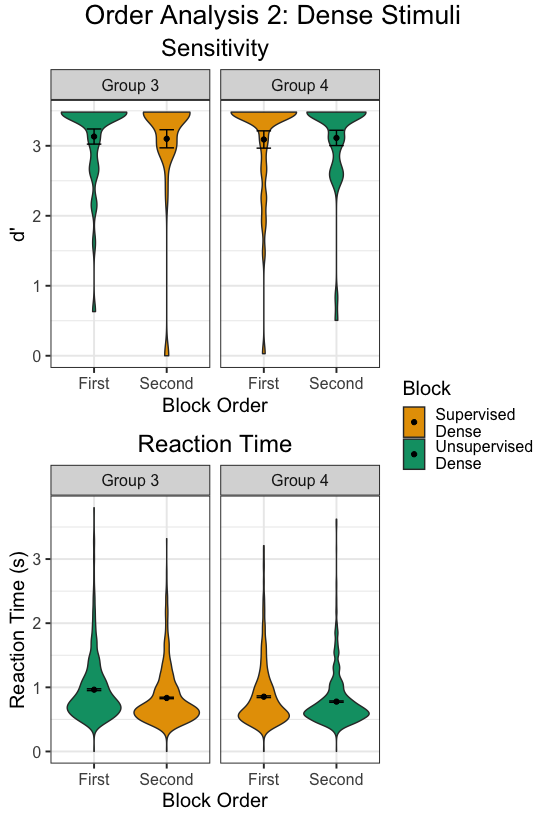
\includegraphics[scale=0.5]{oe2.png}
\caption[Sensitivity and reaction time for order analysis 2]{Sensitivity (d')  and reaction time for each block completed by each group for order analysis 2. Points indicate means with error bars reflecting standard error. Shaded portions represent the distribution of sensitivity or reaction time values.}
\label{oe2}
\vspace{-20pt}
\end{wrapfigure}		
	
	Next, I conducted the individual differences analysis. Since the goal of this investigation was to see whether the relationship between order and sensitivity in each block changed as a function of language ability, I created a model with fixed effects for block, order, and language ability as well as RAM. The model showed no significant effects of any of the predictors. \par 	
	\textbf{Reaction time.} I used the same linear mixed-effects model as above, with random intercepts for subject and for block nested within subject in the base model. Adding fixed effects of order and block did not significantly improve model fit, $\chi^{2}(2)$ = 3.38, \textit{p} = 0.18. Block, \textit{F}(1,71) = 1.12, \textit{p} = 0.29, and order, \textit{F}(1,76) = 2.28, \textit{p} = 0.13, did not have any effect on reaction time. Adding language ability and RAM to the model also did not improve fit. These measures were not significant predictors of reaction time for dense stimuli.\par
	\textbf{Summary (see Fig. \ref{oe2}).} There were no significant effects of block, order, or language ability found for dense stimuli. This may suggest that learning dense stimuli engages a single system regardless of the instructions. Alternatively, it may be that learning dense stimuli is overall an easy task, evidenced by the high sensitivity values seen in these blocks.
	
\subsubsection{Order analysis 3: sparse stimuli}

	The third order analysis investigated differences in learning sparse categories based on learning type order, using data from groups 5 and 6. \par 	
	\textbf{Sensitivity.} I used the same type of linear mixed-effect models as the prior two order effects, with random intercepts for subject. Adding block and order significantly increased model fit, $\chi^{2}(2)$ = 57.5, \textit{p} \textless 0.001. However, adding the interaction between block and order did not increase model fit, $\chi^{2}(1)$ = 0.33, \textit{p} = 0.56. Thus, the final model included fixed effects for order and block but not their interaction. This model revealed a significant main effect of block, \textit{F}(1,67) = 75.69, \textit{p} \textless 0.0001, but no significant main effect of order, \textit{F}(1,67) = 0.0008, \textit{p} = 0.98. Participants showed significantly higher sensitivity in supervised-sparse blocks than in unsupervised-sparse blocks (see Table \ref{exp1expdesc}). \par 
	
\begin{wrapfigure}{R}{0.55\textwidth}
\vspace{-10pt}
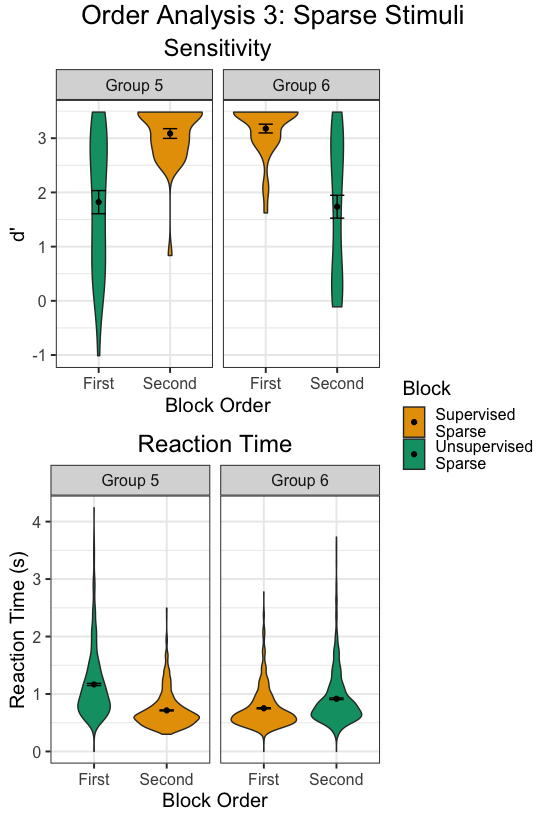
\includegraphics[scale=0.5]{oe3.png}
\caption[Sensitivity and reaction time for order analysis 3]{Sensitivity (d')  and reaction time for each block completed by each group for order analysis 3. Points indicate means with error bars reflecting standard error. Shaded portions represent the distribution of sensitivity or reaction time values.}
\label{oe3}
\vspace{-15pt}
\end{wrapfigure}			
	
	As in the two previous analyses, I added RAM and language ability to the final model above. Adding the language composite improved model fit even after adding RAM, $\chi^{2}(2)$ = 5.34, \textit{p} = 0.02. However, adding the block x language and order x language interactions did not improve model fit, $\chi^{2}(2)$ = 1.94, \textit{p} = 0.38. The final model, which included no interactions, showed the same main effect of block seen above as well as a significant main effect of language ability, \textit{F}(1,63) = 5.21, \textit{p} = 0.03. The effect of language ability was associated with a positive coefficient (\textit{b} = 0.19, \textit{SE} = 0.09), suggesting that sensitivity and language ability were positively related. There was no main effect of RAM. \par 
	
	
\begin{wrapfigure}{L}{0.45\textwidth}
\vspace{-10pt}
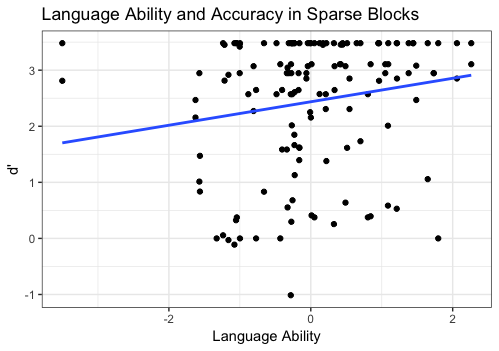
\includegraphics[scale=0.35]{oe3_lang.png}
\caption[Relationship between language ability and accuracy for order analysis 3]{Language ability is a significant predictor of sensitivity (\textit{d'}) for blocks in order analysis 3 (all containing sparse stimuli). }
\label{oe3_lang}
\vspace{-20pt}
\end{wrapfigure}	

	\textbf{Reaction time.} As above, I used a linear mixed-effect model with random intercepts for subject and block nested within subject as the base model. Adding the fixed effects of order and block significantly improved fit, $\chi^{2}(2)$ = 55.08, \textit{p} \textless 0.0001. In addition, adding the interaction between block and order improved fit,  $\chi^{2}(1)$ = 20.00, \textit{p} \textless 0.0001. The final model showed significant main effects for block, \textit{F}(1,68) = 31.22, \textit{p} \textless 0.0001, order, \textit{F}(1,70) = 5.04, \textit{p} = 0.03, and a significant interaction between block and order, \textit{F}(1,68) = 22.25, \textit{p} \textless 0.0001. Follow-up models showed that there was a significant difference in reaction time by block for each order. However, the difference between mean reaction time of the two blocks for group 5 (unsupervised-sparse first) was 415 ms, while the difference for group 6 (supervised-sparse first) was 163 ms. This suggests that the interaction represents a greater difference in reaction time between blocks for participants who received the unsupervised-sparse block first.  \par 
	For the individual differences analysis, I added RAM and the language composite to the final model from above. Adding the language composite did not improve the model fit. There was no effect of language ability on reaction time for sparse stimuli. \par	
	\textbf{Summary (see Fig. \ref{oe3} and Fig. \ref{oe3_lang}).} In terms of accuracy, participants showed higher sensitivity during the supervised-sparse block than during the unsupervised-sparse block, regardless of order. In addition, sensitivity on all blocks was positively related to language ability. This relationship did not vary by block or order. For reaction time, there was an interaction between block and order, but no effect of language ability. The unsupervised-sparse block was by far the most difficult block for all participants who received it. Thus, this interaction may reflect this block difference crossed with learning effects. Participants who received the unsupervised-sparse block second were perhaps more comfortable with the task overall than participants who received the unsupervised-sparse block first, which lead to faster reaction times for those receiving unsupervised-sparse second.

	
\subsection{Discussion}

	In this experiment, I tested three different order effects to see whether the order in which an individual engages the two category learning systems affects their category learning performance. The two manipulations in the statistical density task encouraged participants to use a particular system in two ways (learning type and stimulus type; see Table \ref{stimsystems} for a summary). The first analysis investigated whether block order affected performance when both the learning type engaged and the stimulus type required the same system. The second analysis tested the effect of block order on performance when all stimuli were dense, and the third analysis did the same for only sparse stimuli. \par
	
\subsubsection{Order effects}
	The three analyses revealed what appears to be a general learning effect. It is most apparent in the first analysis, which showed that when both learning type and stimulus type engage the same category learning system, performance is better on the second block than on the first. Group 1 (unsupervised-dense first) showed slower reaction times in their first block, while Group 2 (supervised-sparse first) showed poorer sensitivity in their first block, even though the first block for each of these groups was different. This result was also seen in a block by order interaction in the third analysis, where the difference between blocks in reaction times attenuated when the more difficult block (unsupervised-dense) was encountered second. Finally, while there were no significant effects in the second analysis, the mean reaction times were numerically higher for first blocks than for second. \par
	The core hypothesis for this experiment was that engaging the hypothesis-testing system before the associative system would lead to reduced performance during associative blocks and that the reverse effect would not appear. This hypothesis was based on previous research that showed that when participants were required to switch between categories built using different category rules, they tended to rely more on executive function even if they were not actually switching between rule types \citep{Erickson2008}. Other research also has shown that when participants are asked to learn a hybrid category that combines different rule types, they end up using only a simple rule-based strategy \citep{Ashby2010}. Thus, when individuals are bombarded with cues towards different systems on a trial-to-trial basis, they default to the more explicit strategies, reflecting reliance on the hypothesis-testing system. However, this type of result was not found in the current study. Instead of defaulting to the hypothesis-testing system and thus showing reduced performance on unsupervised or dense blocks that occurred second, better performance was almost always seen in second blocks. This may reflect a broad learning effect that was not seen in prior studies. \par
	Differences in experimental paradigm may at least partially explain why this study shows learning effects while other studies show reliance on a single system. In the studies mentioned above, stimulus characteristics encouraged participants to switch between systems on a trial-by-trial basis. In the current study, trials were blocked and a single system was engaged for that block. Participants had short transition periods between blocks were new instructions and examples or rules were presented. The results presented here suggest that these transition periods were sufficient for participants to switch to a new system as stimulus and task demands changed. 
	
\subsubsection{Individual differences}

	The original hypothesis for this analysis was that individuals with poorer language ability would show stronger order effects than those with better language ability. My prior research has shown that low-language individuals exhibit difficulty switching away from suboptimal learning strategies that were developed in the absence of guided instruction \citep{Ryherd2019}. Thus, I expected to see an interaction between language ability and order such that individuals with better language skills would show minimal costs when switching between unsupervised and supervised tasks, while those with poorer language skills would show a large switch cost. However, no interactions between language ability and order were found. \par
	The third analysis revealed the only significant effect of language ability. This analysis showed that language ability was positively related to sensitivity when all items in both blocks were sparse. Recall that sparse items are best learned by the hypothesis-testing system. Since both blocks in the third order effect analysis were sparse, an individual could succeed by only using this system. The effect of language on category learning is often found only for the hypothesis-testing system \citep{Lupyan2009,Lupyan2013}. Thus, this result is in line with previous findings. \par 
	This finding is especially interesting because it is one of the first to relate category learning performance to individual differences in language ability in an adult sample. This topic has been much more extensively studied in children and infants. For example, vocabulary and  categorization have been shown to be positively correlated in 20-month-olds \citep{Nazzi2001} and 24-month-olds \citep{Jaswal2007}. In addition, infants' categorization ability at 12 months predicts their concurrent and future (18 month) vocabulary size \citep{Ferguson2015}. However, much of the individual differences category learning literature focuses on skills like working memory or strategy use rather than language ability. Thus, this study is one of the first to find that individual differences in language ability are related to categorization accuracy for novel rule-based categories in adults.
	
\subsubsection{Limitations and conclusions}

	While the category learning task used in this study was based off of prior research, it was modified for use in a within-subjects design. To do this, I created different stimuli for each block (see Appendix B). Each stimulus type (e.g, flowers) was tied to a particular block (e.g., supervised-dense). As such, differences between blocks could be due to the specific stimuli that were created. For example, two of the four blocks have animate stimuli (aliens, bugs) while the other two have inanimate stimuli (flags, flowers). Animacy has been shown to affect how children extend category labels \citep{Davidson2018}. Adults also show better memory for animate items than inanimate items \citep{Bonin2014}. This may have contributed to the main effect of system seen in the third order analysis; performance with inanimate items (flags) was worse than performance with animate items (bugs). However, the blocks including inanimate items were unsupervised-sparse, a block type that has been shown to be particularly difficult \citep{Kloos2008}. Considering that similar main effects of block were not seen in the second order analysis, which had a similar animate (alien) vs. inanimate (flower) confound, it is unlikely that animacy affected performance in this task. \par 
	The category learning task would also have benefited from more data on the stimuli themselves. First, it would be helpful to know more about the specific features chosen. The calculations for statistical density include an attentional weight constant which is just assumed to be the same for all features and relations among features. However, this weighting could certainly vary based on the salience of given features (e.g., smiles/frowns may be more salient for friendly/unfriendly aliens), leading to differences in statistical density. Future work would benefit from more extensive norming to fully understand the statistical density of all stimuli. In addition, the task was overall quite easy for the adult sample in this study, leading to some undesired ceiling effects. More complicated stimuli (e.g., more dimensions, disjunctive rules for category membership, etc.) might make the task difficult enough to fully probe category learning in an adult sample. \par
	Despite these limitations, this study contributes to a theoretical understanding of how individuals switch between category learning systems in a blocked design. In addition, it is the first study to test a statistical density category learning paradigm within subjects. The findings suggest that this type of task does not suffer from transfer effects. Instead, participants show modest learning effects, becoming faster and/or more accurate in their second block. These learning effects do not vary by language ability. However, language ability is related to categorization when all stimuli are sparse. Thus, this experiment supports the idea that language ability (broadly defined) is related to categorization in the hypothesis-testing system.
	
\end{document}

